\documentclass[twoside]{book}

% Packages required by doxygen
\usepackage{calc}
\usepackage{doxygen}
\usepackage{graphicx}
\usepackage[utf8]{inputenc}
\usepackage{makeidx}
\usepackage{multicol}
\usepackage{multirow}
\usepackage{textcomp}
\usepackage[table]{xcolor}

% Font selection
\usepackage[T1]{fontenc}
\usepackage{mathptmx}
\usepackage[scaled=.90]{helvet}
\usepackage{courier}
\usepackage{amssymb}
\usepackage{sectsty}
\renewcommand{\familydefault}{\sfdefault}
\allsectionsfont{%
  \fontseries{bc}\selectfont%
  \color{darkgray}%
}
\renewcommand{\DoxyLabelFont}{%
  \fontseries{bc}\selectfont%
  \color{darkgray}%
}

% Page & text layout
\usepackage{geometry}
\geometry{%
  a4paper,%
  top=2.5cm,%
  bottom=2.5cm,%
  left=2.5cm,%
  right=2.5cm%
}
\tolerance=750
\hfuzz=15pt
\hbadness=750
\setlength{\emergencystretch}{15pt}
\setlength{\parindent}{0cm}
\setlength{\parskip}{0.2cm}
\makeatletter
\renewcommand{\paragraph}{%
  \@startsection{paragraph}{4}{0ex}{-1.0ex}{1.0ex}{%
    \normalfont\normalsize\bfseries\SS@parafont%
  }%
}
\renewcommand{\subparagraph}{%
  \@startsection{subparagraph}{5}{0ex}{-1.0ex}{1.0ex}{%
    \normalfont\normalsize\bfseries\SS@subparafont%
  }%
}
\makeatother

% Headers & footers
\usepackage{fancyhdr}
\pagestyle{fancyplain}
\fancyhead[LE]{\fancyplain{}{\bfseries\thepage}}
\fancyhead[CE]{\fancyplain{}{}}
\fancyhead[RE]{\fancyplain{}{\bfseries\leftmark}}
\fancyhead[LO]{\fancyplain{}{\bfseries\rightmark}}
\fancyhead[CO]{\fancyplain{}{}}
\fancyhead[RO]{\fancyplain{}{\bfseries\thepage}}
\fancyfoot[LE]{\fancyplain{}{}}
\fancyfoot[CE]{\fancyplain{}{}}
\fancyfoot[RE]{\fancyplain{}{\bfseries\scriptsize Generated on Sun Mar 29 2020 16\-:49\-:08 for My Project by Doxygen }}
\fancyfoot[LO]{\fancyplain{}{\bfseries\scriptsize Generated on Sun Mar 29 2020 16\-:49\-:08 for My Project by Doxygen }}
\fancyfoot[CO]{\fancyplain{}{}}
\fancyfoot[RO]{\fancyplain{}{}}
\renewcommand{\footrulewidth}{0.4pt}
\renewcommand{\chaptermark}[1]{%
  \markboth{#1}{}%
}
\renewcommand{\sectionmark}[1]{%
  \markright{\thesection\ #1}%
}

% Indices & bibliography
\usepackage{natbib}
\usepackage[titles]{tocloft}
\setcounter{tocdepth}{3}
\setcounter{secnumdepth}{5}
\makeindex

% Hyperlinks (required, but should be loaded last)
\usepackage{ifpdf}
\ifpdf
  \usepackage[pdftex,pagebackref=true]{hyperref}
\else
  \usepackage[ps2pdf,pagebackref=true]{hyperref}
\fi
\hypersetup{%
  colorlinks=true,%
  linkcolor=blue,%
  citecolor=blue,%
  unicode%
}

% Custom commands
\newcommand{\clearemptydoublepage}{%
  \newpage{\pagestyle{empty}\cleardoublepage}%
}


%===== C O N T E N T S =====

\begin{document}

% Titlepage & ToC
\hypersetup{pageanchor=false}
\pagenumbering{roman}
\begin{titlepage}
\vspace*{7cm}
\begin{center}%
{\Large My Project }\\
\vspace*{1cm}
{\large Generated by Doxygen 1.8.5}\\
\vspace*{0.5cm}
{\small Sun Mar 29 2020 16:49:08}\\
\end{center}
\end{titlepage}
\clearemptydoublepage
\tableofcontents
\clearemptydoublepage
\pagenumbering{arabic}
\hypersetup{pageanchor=true}

%--- Begin generated contents ---
\chapter{Hierarchical Index}
\section{Class Hierarchy}
This inheritance list is sorted roughly, but not completely, alphabetically\-:\begin{DoxyCompactList}
\item \contentsline{section}{Appointment\-Slot}{\pageref{classAppointmentSlot}}{}
\item \contentsline{section}{Date}{\pageref{structDate}}{}
\begin{DoxyCompactList}
\item \contentsline{section}{Date\-Time}{\pageref{structDateTime}}{}
\end{DoxyCompactList}
\item \contentsline{section}{Patient}{\pageref{classPatient}}{}
\item \contentsline{section}{Personnel}{\pageref{classPersonnel}}{}
\item \contentsline{section}{Schedule}{\pageref{classSchedule}}{}
\end{DoxyCompactList}

\chapter{Class Index}
\section{Class List}
Here are the classes, structs, unions and interfaces with brief descriptions\-:\begin{DoxyCompactList}
\item\contentsline{section}{\hyperlink{classAppointmentSlot}{Appointment\-Slot} }{\pageref{classAppointmentSlot}}{}
\item\contentsline{section}{\hyperlink{structDate}{Date} }{\pageref{structDate}}{}
\item\contentsline{section}{\hyperlink{structDateTime}{Date\-Time} }{\pageref{structDateTime}}{}
\item\contentsline{section}{\hyperlink{classPatient}{Patient} }{\pageref{classPatient}}{}
\item\contentsline{section}{\hyperlink{classPersonnel}{Personnel} }{\pageref{classPersonnel}}{}
\item\contentsline{section}{\hyperlink{classSchedule}{Schedule} }{\pageref{classSchedule}}{}
\end{DoxyCompactList}

\chapter{Class Documentation}
\hypertarget{classAppointmentSlot}{\section{Appointment\-Slot Class Reference}
\label{classAppointmentSlot}\index{Appointment\-Slot@{Appointment\-Slot}}
}


{\ttfamily \#include $<$Appointment\-Slot.\-h$>$}

\subsection*{Public Member Functions}
\begin{DoxyCompactItemize}
\item 
\hyperlink{structDateTime}{Date\-Time} \hyperlink{classAppointmentSlot_ae1bc0c4c7cdfd6ff0e19dac860ac1795}{get\-Start\-Time} ()
\begin{DoxyCompactList}\small\item\em Retrieve the starting time of the slot. \end{DoxyCompactList}\item 
\hyperlink{structDateTime}{Date\-Time} \hyperlink{classAppointmentSlot_aaabb9dee474cf30db424e4ab84c0f7a8}{get\-End\-Time} ()
\begin{DoxyCompactList}\small\item\em Retrieve the ending time of the slot. \end{DoxyCompactList}\item 
void \hyperlink{classAppointmentSlot_a4e4bad089724bdecf9c71332b34ae50f}{set\-Start\-Time} (\hyperlink{structDateTime}{Date\-Time} start\-Time)
\begin{DoxyCompactList}\small\item\em Set the starting time of the slot. \end{DoxyCompactList}\item 
void \hyperlink{classAppointmentSlot_a2ca48b95d7b9f578f2f23f6d86a7f069}{set\-End\-Time} (\hyperlink{structDateTime}{Date\-Time} end\-Time)
\begin{DoxyCompactList}\small\item\em Set the ending time of the slot. \end{DoxyCompactList}\end{DoxyCompactItemize}


\subsection{Detailed Description}
This class defines the timeslots of appointments, used to mark the times of appointments, personnel working times, and available appointment slots.

\begin{DoxyAuthor}{Author}
Alex Sweeney
\end{DoxyAuthor}
\begin{DoxyVersion}{Version}
1.\-0
\end{DoxyVersion}
Created on Sun Mar 29 2020 

\subsection{Member Function Documentation}
\hypertarget{classAppointmentSlot_aaabb9dee474cf30db424e4ab84c0f7a8}{\index{Appointment\-Slot@{Appointment\-Slot}!get\-End\-Time@{get\-End\-Time}}
\index{get\-End\-Time@{get\-End\-Time}!AppointmentSlot@{Appointment\-Slot}}
\subsubsection[{get\-End\-Time}]{\setlength{\rightskip}{0pt plus 5cm}{\bf Date\-Time} Appointment\-Slot\-::get\-End\-Time (
\begin{DoxyParamCaption}
{}
\end{DoxyParamCaption}
)}}\label{classAppointmentSlot_aaabb9dee474cf30db424e4ab84c0f7a8}


Retrieve the ending time of the slot. 

\begin{DoxyReturn}{Returns}
\hyperlink{structDateTime}{Date\-Time} the ending time of the \hyperlink{classAppointmentSlot}{Appointment\-Slot} 
\end{DoxyReturn}
\hypertarget{classAppointmentSlot_ae1bc0c4c7cdfd6ff0e19dac860ac1795}{\index{Appointment\-Slot@{Appointment\-Slot}!get\-Start\-Time@{get\-Start\-Time}}
\index{get\-Start\-Time@{get\-Start\-Time}!AppointmentSlot@{Appointment\-Slot}}
\subsubsection[{get\-Start\-Time}]{\setlength{\rightskip}{0pt plus 5cm}{\bf Date\-Time} Appointment\-Slot\-::get\-Start\-Time (
\begin{DoxyParamCaption}
{}
\end{DoxyParamCaption}
)}}\label{classAppointmentSlot_ae1bc0c4c7cdfd6ff0e19dac860ac1795}


Retrieve the starting time of the slot. 

\begin{DoxyReturn}{Returns}
\hyperlink{structDateTime}{Date\-Time} the starting time of the \hyperlink{classAppointmentSlot}{Appointment\-Slot} 
\end{DoxyReturn}
\hypertarget{classAppointmentSlot_a2ca48b95d7b9f578f2f23f6d86a7f069}{\index{Appointment\-Slot@{Appointment\-Slot}!set\-End\-Time@{set\-End\-Time}}
\index{set\-End\-Time@{set\-End\-Time}!AppointmentSlot@{Appointment\-Slot}}
\subsubsection[{set\-End\-Time}]{\setlength{\rightskip}{0pt plus 5cm}void Appointment\-Slot\-::set\-End\-Time (
\begin{DoxyParamCaption}
\item[{{\bf Date\-Time}}]{end\-Time}
\end{DoxyParamCaption}
)}}\label{classAppointmentSlot_a2ca48b95d7b9f578f2f23f6d86a7f069}


Set the ending time of the slot. 


\begin{DoxyParams}{Parameters}
{\em end\-Time} & The ending of the appointment \\
\hline
\end{DoxyParams}
\begin{DoxyReturn}{Returns}
none 
\end{DoxyReturn}
\hypertarget{classAppointmentSlot_a4e4bad089724bdecf9c71332b34ae50f}{\index{Appointment\-Slot@{Appointment\-Slot}!set\-Start\-Time@{set\-Start\-Time}}
\index{set\-Start\-Time@{set\-Start\-Time}!AppointmentSlot@{Appointment\-Slot}}
\subsubsection[{set\-Start\-Time}]{\setlength{\rightskip}{0pt plus 5cm}void Appointment\-Slot\-::set\-Start\-Time (
\begin{DoxyParamCaption}
\item[{{\bf Date\-Time}}]{start\-Time}
\end{DoxyParamCaption}
)}}\label{classAppointmentSlot_a4e4bad089724bdecf9c71332b34ae50f}


Set the starting time of the slot. 


\begin{DoxyParams}{Parameters}
{\em start\-Time} & The start of the appointment \\
\hline
\end{DoxyParams}
\begin{DoxyReturn}{Returns}
none 
\end{DoxyReturn}


The documentation for this class was generated from the following file\-:\begin{DoxyCompactItemize}
\item 
Appointment\-Slot.\-h\end{DoxyCompactItemize}

\hypertarget{structDate}{\section{Date Class Reference}
\label{structDate}\index{Date@{Date}}
}


{\ttfamily \#include $<$datetime.\-h$>$}

Inheritance diagram for Date\-:\begin{figure}[H]
\begin{center}
\leavevmode
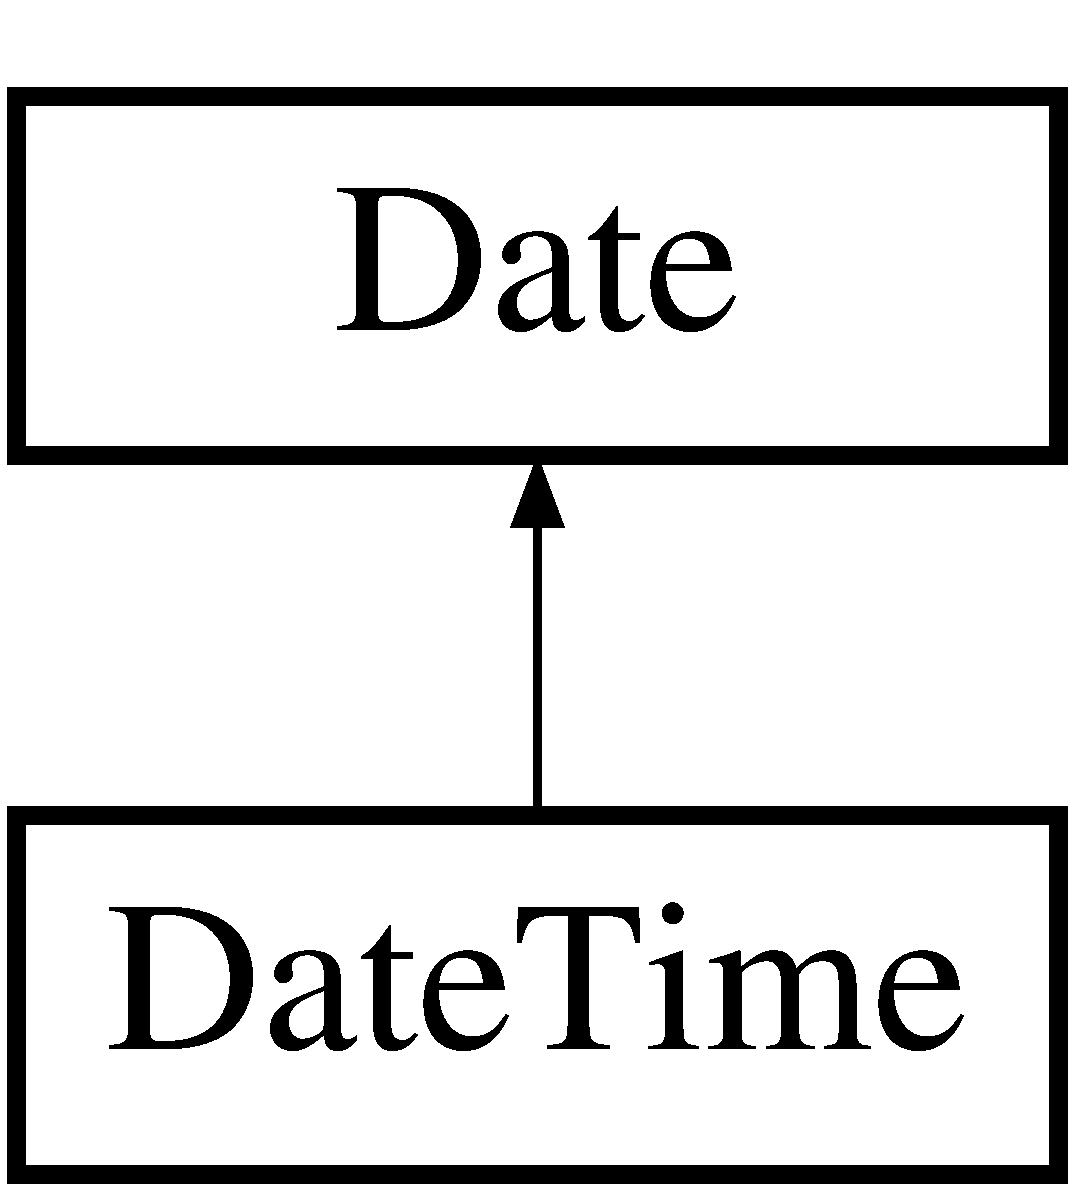
\includegraphics[height=2.000000cm]{structDate}
\end{center}
\end{figure}
\subsection*{Public Attributes}
\begin{DoxyCompactItemize}
\item 
\hypertarget{structDate_a5b192adcabf2b2871e3f0b76c1ec1601}{int \hyperlink{structDate_a5b192adcabf2b2871e3f0b76c1ec1601}{day}}\label{structDate_a5b192adcabf2b2871e3f0b76c1ec1601}

\begin{DoxyCompactList}\small\item\em The day of the month. \end{DoxyCompactList}\item 
\hypertarget{structDate_a533843e07c6ac8d19fee9b16f5336ba2}{int \hyperlink{structDate_a533843e07c6ac8d19fee9b16f5336ba2}{month}}\label{structDate_a533843e07c6ac8d19fee9b16f5336ba2}

\begin{DoxyCompactList}\small\item\em The number of the month. \end{DoxyCompactList}\item 
\hypertarget{structDate_a3eeced2ed56bc95d56782b9e738db8ea}{int \hyperlink{structDate_a3eeced2ed56bc95d56782b9e738db8ea}{year}}\label{structDate_a3eeced2ed56bc95d56782b9e738db8ea}

\begin{DoxyCompactList}\small\item\em The four digit year. \end{DoxyCompactList}\item 
\hypertarget{structDate_a354c151de1d380763cf650f597944485}{string \hyperlink{structDate_a354c151de1d380763cf650f597944485}{day\-Of\-Week}}\label{structDate_a354c151de1d380763cf650f597944485}

\begin{DoxyCompactList}\small\item\em The name of the day of the week. \end{DoxyCompactList}\end{DoxyCompactItemize}


\subsection{Detailed Description}
Defines the \hyperlink{structDate}{Date} objects for appointment slots and other classes, since C++ contains no built-\/in class for this purpose

\begin{DoxyAuthor}{Author}
Alex Sweeney
\end{DoxyAuthor}
\begin{DoxyVersion}{Version}
1.\-0
\end{DoxyVersion}
Created on Sun Mar 29 2020 

The documentation for this class was generated from the following file\-:\begin{DoxyCompactItemize}
\item 
datetime.\-h\end{DoxyCompactItemize}

\hypertarget{structDateTime}{\section{Date\-Time Class Reference}
\label{structDateTime}\index{Date\-Time@{Date\-Time}}
}


{\ttfamily \#include $<$datetime.\-h$>$}

Inheritance diagram for Date\-Time\-:\begin{figure}[H]
\begin{center}
\leavevmode
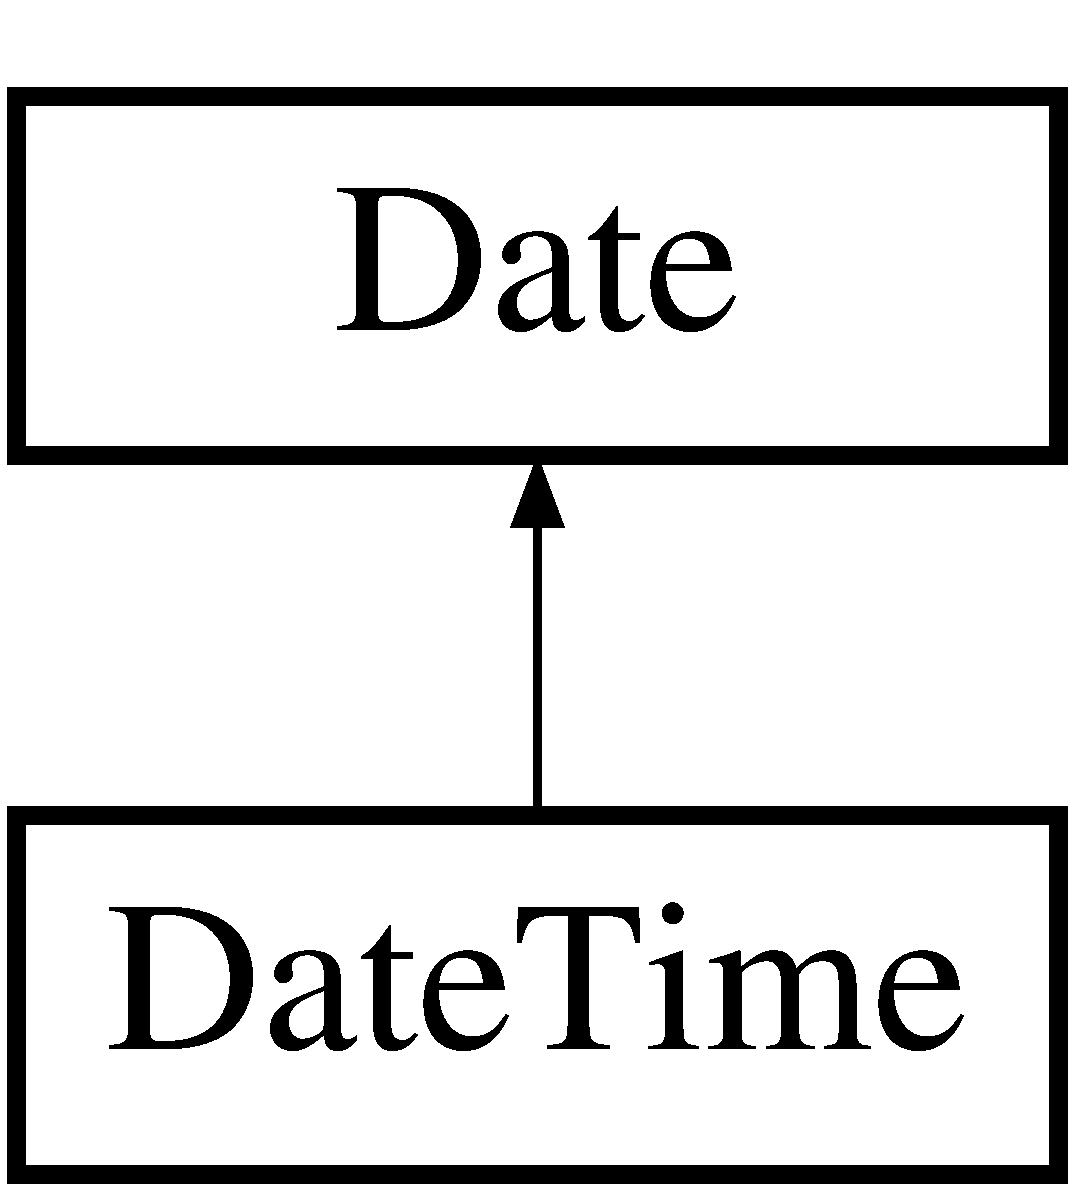
\includegraphics[height=2.000000cm]{structDateTime}
\end{center}
\end{figure}
\subsection*{Public Attributes}
\begin{DoxyCompactItemize}
\item 
\hypertarget{structDateTime_a870c42c1a64681bcc8b67d57a5c9d53b}{int \hyperlink{structDateTime_a870c42c1a64681bcc8b67d57a5c9d53b}{hour}}\label{structDateTime_a870c42c1a64681bcc8b67d57a5c9d53b}

\begin{DoxyCompactList}\small\item\em The number of the hour (24h clock) \end{DoxyCompactList}\item 
\hypertarget{structDateTime_a968aece0ae2649712e90d93d4613e08f}{int \hyperlink{structDateTime_a968aece0ae2649712e90d93d4613e08f}{minute}}\label{structDateTime_a968aece0ae2649712e90d93d4613e08f}

\begin{DoxyCompactList}\small\item\em The number of the minute. \end{DoxyCompactList}\item 
\hypertarget{structDateTime_a0b36196a591d08b2512b02f7058560ee}{int \hyperlink{structDateTime_a0b36196a591d08b2512b02f7058560ee}{seconds}}\label{structDateTime_a0b36196a591d08b2512b02f7058560ee}

\begin{DoxyCompactList}\small\item\em The number of seconds. \end{DoxyCompactList}\end{DoxyCompactItemize}


\subsection{Detailed Description}
Defines the \hyperlink{structDateTime}{Date\-Time} objects for appointment slots and other classes, since C++ contains no built-\/in class for this purpose. Inherits from \hyperlink{structDate}{Date} and adds the time attributes

\begin{DoxyAuthor}{Author}
Alex Sweeney
\end{DoxyAuthor}
\begin{DoxyVersion}{Version}
1.\-0
\end{DoxyVersion}
Created on Sun Mar 29 2020 

The documentation for this class was generated from the following file\-:\begin{DoxyCompactItemize}
\item 
datetime.\-h\end{DoxyCompactItemize}

\hypertarget{classPatient}{\section{Patient Class Reference}
\label{classPatient}\index{Patient@{Patient}}
}


{\ttfamily \#include $<$Patient.\-h$>$}

\subsection*{Public Member Functions}
\begin{DoxyCompactItemize}
\item 
string \hyperlink{classPatient_a69910a374b455ce5c5f148a93279d9cf}{get\-Name} ()
\begin{DoxyCompactList}\small\item\em Retrieve the name of the patient. \end{DoxyCompactList}\item 
string \hyperlink{classPatient_a09f45cf60eb7d32b63e4002f6215c57f}{get\-Gender} ()
\begin{DoxyCompactList}\small\item\em Retrieve the gender of the patient. \end{DoxyCompactList}\item 
string \hyperlink{classPatient_a6a7acd37be18d10dc278e9a73be88a82}{get\-Race} ()
\begin{DoxyCompactList}\small\item\em Retrieve the race of the patient. \end{DoxyCompactList}\item 
string \hyperlink{classPatient_a74ff6cd63c820abe325b6255723074f0}{get\-Patient\-Type} ()
\begin{DoxyCompactList}\small\item\em Retrieve the type of the patient. \end{DoxyCompactList}\item 
\hyperlink{structDate}{Date} \hyperlink{classPatient_a1ef2aa700d64adfc6dae6e32b2f2325c}{get\-Dob} ()
\begin{DoxyCompactList}\small\item\em Retrieve the date of birth of the patient. \end{DoxyCompactList}\item 
int \hyperlink{classPatient_a86847067f9dfc59e5a86229a5a9e6ea8}{get\-K\-S\-U\-I\-D} ()
\begin{DoxyCompactList}\small\item\em Retrieve the K\-S\-U I\-D of the patient. \end{DoxyCompactList}\item 
void \hyperlink{classPatient_ae2a86b85bcc96d524aa3cdf8e3b4eb1d}{set\-Patient\-Type} (string patienttype)
\begin{DoxyCompactList}\small\item\em Set the type of the patient. \end{DoxyCompactList}\item 
void \hyperlink{classPatient_a2e46826f0c95fdf8f6f1f4f685176658}{set\-Name} (string name)
\begin{DoxyCompactList}\small\item\em Set the full name of the patient. \end{DoxyCompactList}\item 
void \hyperlink{classPatient_a1db1579eb65b1c33e01319cd96ed5249}{set\-K\-S\-U\-I\-D} (int ksu\-I\-D)
\begin{DoxyCompactList}\small\item\em Set the K\-S\-U I\-D of the patient. \end{DoxyCompactList}\item 
void \hyperlink{classPatient_a83af64a0500ef639cd11a610c1fce357}{set\-Gender} (string gender)
\begin{DoxyCompactList}\small\item\em Set the gender of the patient. \end{DoxyCompactList}\item 
void \hyperlink{classPatient_a24138f2d4c26928048a5af538a18d7fb}{set\-Dob} (\hyperlink{structDate}{Date} dob)
\begin{DoxyCompactList}\small\item\em Set the date of birth of the patient. \end{DoxyCompactList}\item 
void \hyperlink{classPatient_ab1f73f7a754d309d4cdff9a38784819c}{set\-Race} (string race)
\begin{DoxyCompactList}\small\item\em Set the race of the patient. \end{DoxyCompactList}\end{DoxyCompactItemize}


\subsection{Detailed Description}
This class defines the object to store patient data.

\begin{DoxyAuthor}{Author}
Alex Sweeney
\end{DoxyAuthor}
\begin{DoxyVersion}{Version}
1.\-0
\end{DoxyVersion}
Created on Sun Mar 29 2020 

\subsection{Member Function Documentation}
\hypertarget{classPatient_a1ef2aa700d64adfc6dae6e32b2f2325c}{\index{Patient@{Patient}!get\-Dob@{get\-Dob}}
\index{get\-Dob@{get\-Dob}!Patient@{Patient}}
\subsubsection[{get\-Dob}]{\setlength{\rightskip}{0pt plus 5cm}{\bf Date} Patient\-::get\-Dob (
\begin{DoxyParamCaption}
{}
\end{DoxyParamCaption}
)}}\label{classPatient_a1ef2aa700d64adfc6dae6e32b2f2325c}


Retrieve the date of birth of the patient. 

\begin{DoxyReturn}{Returns}
\hyperlink{structDate}{Date} The date of birth of the patient 
\end{DoxyReturn}
\hypertarget{classPatient_a09f45cf60eb7d32b63e4002f6215c57f}{\index{Patient@{Patient}!get\-Gender@{get\-Gender}}
\index{get\-Gender@{get\-Gender}!Patient@{Patient}}
\subsubsection[{get\-Gender}]{\setlength{\rightskip}{0pt plus 5cm}string Patient\-::get\-Gender (
\begin{DoxyParamCaption}
{}
\end{DoxyParamCaption}
)}}\label{classPatient_a09f45cf60eb7d32b63e4002f6215c57f}


Retrieve the gender of the patient. 

\begin{DoxyReturn}{Returns}
string The gender of the patient 
\end{DoxyReturn}
\hypertarget{classPatient_a86847067f9dfc59e5a86229a5a9e6ea8}{\index{Patient@{Patient}!get\-K\-S\-U\-I\-D@{get\-K\-S\-U\-I\-D}}
\index{get\-K\-S\-U\-I\-D@{get\-K\-S\-U\-I\-D}!Patient@{Patient}}
\subsubsection[{get\-K\-S\-U\-I\-D}]{\setlength{\rightskip}{0pt plus 5cm}int Patient\-::get\-K\-S\-U\-I\-D (
\begin{DoxyParamCaption}
{}
\end{DoxyParamCaption}
)}}\label{classPatient_a86847067f9dfc59e5a86229a5a9e6ea8}


Retrieve the K\-S\-U I\-D of the patient. 

\begin{DoxyReturn}{Returns}
int The K\-S\-U I\-D of the patient 
\end{DoxyReturn}
\hypertarget{classPatient_a69910a374b455ce5c5f148a93279d9cf}{\index{Patient@{Patient}!get\-Name@{get\-Name}}
\index{get\-Name@{get\-Name}!Patient@{Patient}}
\subsubsection[{get\-Name}]{\setlength{\rightskip}{0pt plus 5cm}string Patient\-::get\-Name (
\begin{DoxyParamCaption}
{}
\end{DoxyParamCaption}
)}}\label{classPatient_a69910a374b455ce5c5f148a93279d9cf}


Retrieve the name of the patient. 

\begin{DoxyReturn}{Returns}
string The full name of the patient 
\end{DoxyReturn}
\hypertarget{classPatient_a74ff6cd63c820abe325b6255723074f0}{\index{Patient@{Patient}!get\-Patient\-Type@{get\-Patient\-Type}}
\index{get\-Patient\-Type@{get\-Patient\-Type}!Patient@{Patient}}
\subsubsection[{get\-Patient\-Type}]{\setlength{\rightskip}{0pt plus 5cm}string Patient\-::get\-Patient\-Type (
\begin{DoxyParamCaption}
{}
\end{DoxyParamCaption}
)}}\label{classPatient_a74ff6cd63c820abe325b6255723074f0}


Retrieve the type of the patient. 

\begin{DoxyReturn}{Returns}
string The type of the patient 
\end{DoxyReturn}
\hypertarget{classPatient_a6a7acd37be18d10dc278e9a73be88a82}{\index{Patient@{Patient}!get\-Race@{get\-Race}}
\index{get\-Race@{get\-Race}!Patient@{Patient}}
\subsubsection[{get\-Race}]{\setlength{\rightskip}{0pt plus 5cm}string Patient\-::get\-Race (
\begin{DoxyParamCaption}
{}
\end{DoxyParamCaption}
)}}\label{classPatient_a6a7acd37be18d10dc278e9a73be88a82}


Retrieve the race of the patient. 

\begin{DoxyReturn}{Returns}
string The race of the patient 
\end{DoxyReturn}
\hypertarget{classPatient_a24138f2d4c26928048a5af538a18d7fb}{\index{Patient@{Patient}!set\-Dob@{set\-Dob}}
\index{set\-Dob@{set\-Dob}!Patient@{Patient}}
\subsubsection[{set\-Dob}]{\setlength{\rightskip}{0pt plus 5cm}void Patient\-::set\-Dob (
\begin{DoxyParamCaption}
\item[{{\bf Date}}]{dob}
\end{DoxyParamCaption}
)}}\label{classPatient_a24138f2d4c26928048a5af538a18d7fb}


Set the date of birth of the patient. 


\begin{DoxyParams}{Parameters}
{\em dob} & The date of birth of the patient \\
\hline
\end{DoxyParams}
\begin{DoxyReturn}{Returns}
none 
\end{DoxyReturn}
\hypertarget{classPatient_a83af64a0500ef639cd11a610c1fce357}{\index{Patient@{Patient}!set\-Gender@{set\-Gender}}
\index{set\-Gender@{set\-Gender}!Patient@{Patient}}
\subsubsection[{set\-Gender}]{\setlength{\rightskip}{0pt plus 5cm}void Patient\-::set\-Gender (
\begin{DoxyParamCaption}
\item[{string}]{gender}
\end{DoxyParamCaption}
)}}\label{classPatient_a83af64a0500ef639cd11a610c1fce357}


Set the gender of the patient. 


\begin{DoxyParams}{Parameters}
{\em gender} & The gender of the patient \\
\hline
\end{DoxyParams}
\begin{DoxyReturn}{Returns}
none 
\end{DoxyReturn}
\hypertarget{classPatient_a1db1579eb65b1c33e01319cd96ed5249}{\index{Patient@{Patient}!set\-K\-S\-U\-I\-D@{set\-K\-S\-U\-I\-D}}
\index{set\-K\-S\-U\-I\-D@{set\-K\-S\-U\-I\-D}!Patient@{Patient}}
\subsubsection[{set\-K\-S\-U\-I\-D}]{\setlength{\rightskip}{0pt plus 5cm}void Patient\-::set\-K\-S\-U\-I\-D (
\begin{DoxyParamCaption}
\item[{int}]{ksu\-I\-D}
\end{DoxyParamCaption}
)}}\label{classPatient_a1db1579eb65b1c33e01319cd96ed5249}


Set the K\-S\-U I\-D of the patient. 


\begin{DoxyParams}{Parameters}
{\em ksu\-I\-D} & The K\-S\-U I\-D of the patient \\
\hline
\end{DoxyParams}
\begin{DoxyReturn}{Returns}
none 
\end{DoxyReturn}
\hypertarget{classPatient_a2e46826f0c95fdf8f6f1f4f685176658}{\index{Patient@{Patient}!set\-Name@{set\-Name}}
\index{set\-Name@{set\-Name}!Patient@{Patient}}
\subsubsection[{set\-Name}]{\setlength{\rightskip}{0pt plus 5cm}void Patient\-::set\-Name (
\begin{DoxyParamCaption}
\item[{string}]{name}
\end{DoxyParamCaption}
)}}\label{classPatient_a2e46826f0c95fdf8f6f1f4f685176658}


Set the full name of the patient. 


\begin{DoxyParams}{Parameters}
{\em name} & The full name of the patient \\
\hline
\end{DoxyParams}
\begin{DoxyReturn}{Returns}
none 
\end{DoxyReturn}
\hypertarget{classPatient_ae2a86b85bcc96d524aa3cdf8e3b4eb1d}{\index{Patient@{Patient}!set\-Patient\-Type@{set\-Patient\-Type}}
\index{set\-Patient\-Type@{set\-Patient\-Type}!Patient@{Patient}}
\subsubsection[{set\-Patient\-Type}]{\setlength{\rightskip}{0pt plus 5cm}void Patient\-::set\-Patient\-Type (
\begin{DoxyParamCaption}
\item[{string}]{patienttype}
\end{DoxyParamCaption}
)}}\label{classPatient_ae2a86b85bcc96d524aa3cdf8e3b4eb1d}


Set the type of the patient. 


\begin{DoxyParams}{Parameters}
{\em patienttype} & The type of the patient \\
\hline
\end{DoxyParams}
\begin{DoxyReturn}{Returns}
none 
\end{DoxyReturn}
\hypertarget{classPatient_ab1f73f7a754d309d4cdff9a38784819c}{\index{Patient@{Patient}!set\-Race@{set\-Race}}
\index{set\-Race@{set\-Race}!Patient@{Patient}}
\subsubsection[{set\-Race}]{\setlength{\rightskip}{0pt plus 5cm}void Patient\-::set\-Race (
\begin{DoxyParamCaption}
\item[{string}]{race}
\end{DoxyParamCaption}
)}}\label{classPatient_ab1f73f7a754d309d4cdff9a38784819c}


Set the race of the patient. 


\begin{DoxyParams}{Parameters}
{\em race} & The race of the patient \\
\hline
\end{DoxyParams}
\begin{DoxyReturn}{Returns}
none 
\end{DoxyReturn}


The documentation for this class was generated from the following file\-:\begin{DoxyCompactItemize}
\item 
Patient.\-h\end{DoxyCompactItemize}

\hypertarget{classPersonnel}{\section{Personnel Class Reference}
\label{classPersonnel}\index{Personnel@{Personnel}}
}


{\ttfamily \#include $<$Personnel.\-h$>$}

\subsection*{Public Member Functions}
\begin{DoxyCompactItemize}
\item 
string \hyperlink{classPersonnel_afa3b060fdfe99c2b5b5a639f8f23af36}{get\-Name} ()
\begin{DoxyCompactList}\small\item\em Retrieve the name of the personnel. \end{DoxyCompactList}\item 
string \hyperlink{classPersonnel_adb147189db398cfba7af263375976810}{get\-Type} ()
\begin{DoxyCompactList}\small\item\em Retrieve the type of the personnel. \end{DoxyCompactList}\item 
int \hyperlink{classPersonnel_a2e591b54342e4e6231188a7edfb5bc29}{get\-Employee\-Id} ()
\begin{DoxyCompactList}\small\item\em Retrieve the id of the personnel. \end{DoxyCompactList}\item 
\hyperlink{classAppointmentSlot}{Appointment\-Slot} $\ast$ \hyperlink{classPersonnel_afe87cfc23870c19edbc9b0b9b2a076c7}{get\-Working\-Times} ()
\begin{DoxyCompactList}\small\item\em Retrieve the schedule of the personnel. \end{DoxyCompactList}\item 
void \hyperlink{classPersonnel_a0ebbd3ea047e1c88d9385c92a01b9038}{set\-Type} (string type)
\begin{DoxyCompactList}\small\item\em Set the type of the personnel. \end{DoxyCompactList}\item 
void \hyperlink{classPersonnel_a1b8bbd0a1bbd19b527732f1b5e4ced78}{set\-Name} (string name)
\begin{DoxyCompactList}\small\item\em Set the name of the personnel. \end{DoxyCompactList}\item 
void \hyperlink{classPersonnel_a46158f3ea7b0bfe08df92d80f8f6e28e}{set\-Employee\-Id} (int employee\-I\-D)
\begin{DoxyCompactList}\small\item\em Set the id of the personnel. \end{DoxyCompactList}\item 
void \hyperlink{classPersonnel_a6e1c9dcfd49f56b6f0bde128ec2e0725}{add\-Working\-Time} (\hyperlink{classAppointmentSlot}{Appointment\-Slot} work\-Time)
\begin{DoxyCompactList}\small\item\em Add a working time of the personnel. \end{DoxyCompactList}\end{DoxyCompactItemize}


\subsection{Detailed Description}
Defines the object of an employee of the K\-S\-U health services that provides care

\begin{DoxyAuthor}{Author}
Alex Sweeney
\end{DoxyAuthor}
\begin{DoxyVersion}{Version}
1.\-0
\end{DoxyVersion}
Created on Sun Mar 29 2020 

\subsection{Member Function Documentation}
\hypertarget{classPersonnel_a6e1c9dcfd49f56b6f0bde128ec2e0725}{\index{Personnel@{Personnel}!add\-Working\-Time@{add\-Working\-Time}}
\index{add\-Working\-Time@{add\-Working\-Time}!Personnel@{Personnel}}
\subsubsection[{add\-Working\-Time}]{\setlength{\rightskip}{0pt plus 5cm}void Personnel\-::add\-Working\-Time (
\begin{DoxyParamCaption}
\item[{{\bf Appointment\-Slot}}]{work\-Time}
\end{DoxyParamCaption}
)}}\label{classPersonnel_a6e1c9dcfd49f56b6f0bde128ec2e0725}


Add a working time of the personnel. 


\begin{DoxyParams}{Parameters}
{\em work\-Time} & The working time of the personnel \\
\hline
\end{DoxyParams}
\begin{DoxyReturn}{Returns}
none 
\end{DoxyReturn}
\hypertarget{classPersonnel_a2e591b54342e4e6231188a7edfb5bc29}{\index{Personnel@{Personnel}!get\-Employee\-Id@{get\-Employee\-Id}}
\index{get\-Employee\-Id@{get\-Employee\-Id}!Personnel@{Personnel}}
\subsubsection[{get\-Employee\-Id}]{\setlength{\rightskip}{0pt plus 5cm}int Personnel\-::get\-Employee\-Id (
\begin{DoxyParamCaption}
{}
\end{DoxyParamCaption}
)}}\label{classPersonnel_a2e591b54342e4e6231188a7edfb5bc29}


Retrieve the id of the personnel. 

\begin{DoxyReturn}{Returns}
int The id of the personnel 
\end{DoxyReturn}
\hypertarget{classPersonnel_afa3b060fdfe99c2b5b5a639f8f23af36}{\index{Personnel@{Personnel}!get\-Name@{get\-Name}}
\index{get\-Name@{get\-Name}!Personnel@{Personnel}}
\subsubsection[{get\-Name}]{\setlength{\rightskip}{0pt plus 5cm}string Personnel\-::get\-Name (
\begin{DoxyParamCaption}
{}
\end{DoxyParamCaption}
)}}\label{classPersonnel_afa3b060fdfe99c2b5b5a639f8f23af36}


Retrieve the name of the personnel. 

\begin{DoxyReturn}{Returns}
string The name of the personnel 
\end{DoxyReturn}
\hypertarget{classPersonnel_adb147189db398cfba7af263375976810}{\index{Personnel@{Personnel}!get\-Type@{get\-Type}}
\index{get\-Type@{get\-Type}!Personnel@{Personnel}}
\subsubsection[{get\-Type}]{\setlength{\rightskip}{0pt plus 5cm}string Personnel\-::get\-Type (
\begin{DoxyParamCaption}
{}
\end{DoxyParamCaption}
)}}\label{classPersonnel_adb147189db398cfba7af263375976810}


Retrieve the type of the personnel. 

\begin{DoxyReturn}{Returns}
string The type of the personnel 
\end{DoxyReturn}
\hypertarget{classPersonnel_afe87cfc23870c19edbc9b0b9b2a076c7}{\index{Personnel@{Personnel}!get\-Working\-Times@{get\-Working\-Times}}
\index{get\-Working\-Times@{get\-Working\-Times}!Personnel@{Personnel}}
\subsubsection[{get\-Working\-Times}]{\setlength{\rightskip}{0pt plus 5cm}{\bf Appointment\-Slot}$\ast$ Personnel\-::get\-Working\-Times (
\begin{DoxyParamCaption}
{}
\end{DoxyParamCaption}
)}}\label{classPersonnel_afe87cfc23870c19edbc9b0b9b2a076c7}


Retrieve the schedule of the personnel. 

\begin{DoxyReturn}{Returns}
Appointment\-Slot$\ast$ The schedule of the personnel 
\end{DoxyReturn}
\hypertarget{classPersonnel_a46158f3ea7b0bfe08df92d80f8f6e28e}{\index{Personnel@{Personnel}!set\-Employee\-Id@{set\-Employee\-Id}}
\index{set\-Employee\-Id@{set\-Employee\-Id}!Personnel@{Personnel}}
\subsubsection[{set\-Employee\-Id}]{\setlength{\rightskip}{0pt plus 5cm}void Personnel\-::set\-Employee\-Id (
\begin{DoxyParamCaption}
\item[{int}]{employee\-I\-D}
\end{DoxyParamCaption}
)}}\label{classPersonnel_a46158f3ea7b0bfe08df92d80f8f6e28e}


Set the id of the personnel. 


\begin{DoxyParams}{Parameters}
{\em employee\-I\-D} & The id of the personnel \\
\hline
\end{DoxyParams}
\begin{DoxyReturn}{Returns}
none 
\end{DoxyReturn}
\hypertarget{classPersonnel_a1b8bbd0a1bbd19b527732f1b5e4ced78}{\index{Personnel@{Personnel}!set\-Name@{set\-Name}}
\index{set\-Name@{set\-Name}!Personnel@{Personnel}}
\subsubsection[{set\-Name}]{\setlength{\rightskip}{0pt plus 5cm}void Personnel\-::set\-Name (
\begin{DoxyParamCaption}
\item[{string}]{name}
\end{DoxyParamCaption}
)}}\label{classPersonnel_a1b8bbd0a1bbd19b527732f1b5e4ced78}


Set the name of the personnel. 


\begin{DoxyParams}{Parameters}
{\em name} & The name of the personnel \\
\hline
\end{DoxyParams}
\begin{DoxyReturn}{Returns}
none 
\end{DoxyReturn}
\hypertarget{classPersonnel_a0ebbd3ea047e1c88d9385c92a01b9038}{\index{Personnel@{Personnel}!set\-Type@{set\-Type}}
\index{set\-Type@{set\-Type}!Personnel@{Personnel}}
\subsubsection[{set\-Type}]{\setlength{\rightskip}{0pt plus 5cm}void Personnel\-::set\-Type (
\begin{DoxyParamCaption}
\item[{string}]{type}
\end{DoxyParamCaption}
)}}\label{classPersonnel_a0ebbd3ea047e1c88d9385c92a01b9038}


Set the type of the personnel. 


\begin{DoxyParams}{Parameters}
{\em type} & The type of the personnel \\
\hline
\end{DoxyParams}
\begin{DoxyReturn}{Returns}
none 
\end{DoxyReturn}


The documentation for this class was generated from the following file\-:\begin{DoxyCompactItemize}
\item 
Personnel.\-h\end{DoxyCompactItemize}

\hypertarget{classSchedule}{\section{Schedule Class Reference}
\label{classSchedule}\index{Schedule@{Schedule}}
}


{\ttfamily \#include $<$Schedule.\-h$>$}

\subsection*{Public Member Functions}
\begin{DoxyCompactItemize}
\item 
\hyperlink{structDate}{Date} \hyperlink{classSchedule_afdf91c885aeba022140a9cfb5a9c1ba4}{get\-Date} ()
\begin{DoxyCompactList}\small\item\em Retrieve the date the schedule is for. \end{DoxyCompactList}\item 
Appointment $\ast$ \hyperlink{classSchedule_a86714dcdba5007e5627fd07996bd64ea}{get\-Appointments} ()
\begin{DoxyCompactList}\small\item\em Retrieve the currently booked appointments. \end{DoxyCompactList}\item 
\hyperlink{classAppointmentSlot}{Appointment\-Slot} $\ast$ \hyperlink{classSchedule_a621cc493f30f6b4aa5de332b0e60c800}{get\-Available\-Slots} ()
\begin{DoxyCompactList}\small\item\em Retrieve the currently available slots. \end{DoxyCompactList}\item 
void \hyperlink{classSchedule_a218335a66a3e2345dc249e7c951aa437}{set\-Date} (\hyperlink{structDate}{Date} date)
\begin{DoxyCompactList}\small\item\em Set the date of the appointment. \end{DoxyCompactList}\item 
void \hyperlink{classSchedule_a8406c2157c04cfdc6b6946ab0a2ab6cb}{add\-Appointment} (Appointment appointment)
\begin{DoxyCompactList}\small\item\em Add an appointment to the booked appointments. \end{DoxyCompactList}\item 
void \hyperlink{classSchedule_ac0cc730d87aedb39a7ed1e6ea9dc4ba7}{remove\-Appointment} (Appointment appointment)
\begin{DoxyCompactList}\small\item\em Remove an appointment to the booked appointments. \end{DoxyCompactList}\item 
void \hyperlink{classSchedule_a91f472317535422af1fa0e8304e4ca1b}{add\-Available\-Slot} (\hyperlink{classAppointmentSlot}{Appointment\-Slot} slot)
\begin{DoxyCompactList}\small\item\em Add an Appointment Slot to the available Appointment Slots. \end{DoxyCompactList}\item 
void \hyperlink{classSchedule_a1487df95f4fb4f5324c76f20b7a444b4}{remove\-Available\-Slot} (\hyperlink{classAppointmentSlot}{Appointment\-Slot} slot)
\begin{DoxyCompactList}\small\item\em Remove an Appointment Slot to the available Appointment Slots. \end{DoxyCompactList}\end{DoxyCompactItemize}


\subsection{Detailed Description}
Defines the daily schedule of appointments

\begin{DoxyAuthor}{Author}
Alex Sweeney
\end{DoxyAuthor}
\begin{DoxyVersion}{Version}
1.\-0
\end{DoxyVersion}
Created on Sun Mar 29 2020 

\subsection{Member Function Documentation}
\hypertarget{classSchedule_a8406c2157c04cfdc6b6946ab0a2ab6cb}{\index{Schedule@{Schedule}!add\-Appointment@{add\-Appointment}}
\index{add\-Appointment@{add\-Appointment}!Schedule@{Schedule}}
\subsubsection[{add\-Appointment}]{\setlength{\rightskip}{0pt plus 5cm}void Schedule\-::add\-Appointment (
\begin{DoxyParamCaption}
\item[{Appointment}]{appointment}
\end{DoxyParamCaption}
)}}\label{classSchedule_a8406c2157c04cfdc6b6946ab0a2ab6cb}


Add an appointment to the booked appointments. 


\begin{DoxyParams}{Parameters}
{\em appointment} & The appointment to add \\
\hline
\end{DoxyParams}
\begin{DoxyReturn}{Returns}
none 
\end{DoxyReturn}
\hypertarget{classSchedule_a91f472317535422af1fa0e8304e4ca1b}{\index{Schedule@{Schedule}!add\-Available\-Slot@{add\-Available\-Slot}}
\index{add\-Available\-Slot@{add\-Available\-Slot}!Schedule@{Schedule}}
\subsubsection[{add\-Available\-Slot}]{\setlength{\rightskip}{0pt plus 5cm}void Schedule\-::add\-Available\-Slot (
\begin{DoxyParamCaption}
\item[{{\bf Appointment\-Slot}}]{slot}
\end{DoxyParamCaption}
)}}\label{classSchedule_a91f472317535422af1fa0e8304e4ca1b}


Add an Appointment Slot to the available Appointment Slots. 


\begin{DoxyParams}{Parameters}
{\em slot} & The \hyperlink{classAppointmentSlot}{Appointment\-Slot} to add \\
\hline
\end{DoxyParams}
\begin{DoxyReturn}{Returns}
none 
\end{DoxyReturn}
\hypertarget{classSchedule_a86714dcdba5007e5627fd07996bd64ea}{\index{Schedule@{Schedule}!get\-Appointments@{get\-Appointments}}
\index{get\-Appointments@{get\-Appointments}!Schedule@{Schedule}}
\subsubsection[{get\-Appointments}]{\setlength{\rightskip}{0pt plus 5cm}Appointment$\ast$ Schedule\-::get\-Appointments (
\begin{DoxyParamCaption}
{}
\end{DoxyParamCaption}
)}}\label{classSchedule_a86714dcdba5007e5627fd07996bd64ea}


Retrieve the currently booked appointments. 

\begin{DoxyReturn}{Returns}
Appointment$\ast$ The currently booked appointments 
\end{DoxyReturn}
\hypertarget{classSchedule_a621cc493f30f6b4aa5de332b0e60c800}{\index{Schedule@{Schedule}!get\-Available\-Slots@{get\-Available\-Slots}}
\index{get\-Available\-Slots@{get\-Available\-Slots}!Schedule@{Schedule}}
\subsubsection[{get\-Available\-Slots}]{\setlength{\rightskip}{0pt plus 5cm}{\bf Appointment\-Slot}$\ast$ Schedule\-::get\-Available\-Slots (
\begin{DoxyParamCaption}
{}
\end{DoxyParamCaption}
)}}\label{classSchedule_a621cc493f30f6b4aa5de332b0e60c800}


Retrieve the currently available slots. 

\begin{DoxyReturn}{Returns}
Appointment\-Slot$\ast$ The currently available slots 
\end{DoxyReturn}
\hypertarget{classSchedule_afdf91c885aeba022140a9cfb5a9c1ba4}{\index{Schedule@{Schedule}!get\-Date@{get\-Date}}
\index{get\-Date@{get\-Date}!Schedule@{Schedule}}
\subsubsection[{get\-Date}]{\setlength{\rightskip}{0pt plus 5cm}{\bf Date} Schedule\-::get\-Date (
\begin{DoxyParamCaption}
{}
\end{DoxyParamCaption}
)}}\label{classSchedule_afdf91c885aeba022140a9cfb5a9c1ba4}


Retrieve the date the schedule is for. 

\begin{DoxyReturn}{Returns}
\hyperlink{structDate}{Date} the date the schedule is for 
\end{DoxyReturn}
\hypertarget{classSchedule_ac0cc730d87aedb39a7ed1e6ea9dc4ba7}{\index{Schedule@{Schedule}!remove\-Appointment@{remove\-Appointment}}
\index{remove\-Appointment@{remove\-Appointment}!Schedule@{Schedule}}
\subsubsection[{remove\-Appointment}]{\setlength{\rightskip}{0pt plus 5cm}void Schedule\-::remove\-Appointment (
\begin{DoxyParamCaption}
\item[{Appointment}]{appointment}
\end{DoxyParamCaption}
)}}\label{classSchedule_ac0cc730d87aedb39a7ed1e6ea9dc4ba7}


Remove an appointment to the booked appointments. 


\begin{DoxyParams}{Parameters}
{\em appointment} & The appointment to remove \\
\hline
\end{DoxyParams}
\begin{DoxyReturn}{Returns}
none 
\end{DoxyReturn}
\hypertarget{classSchedule_a1487df95f4fb4f5324c76f20b7a444b4}{\index{Schedule@{Schedule}!remove\-Available\-Slot@{remove\-Available\-Slot}}
\index{remove\-Available\-Slot@{remove\-Available\-Slot}!Schedule@{Schedule}}
\subsubsection[{remove\-Available\-Slot}]{\setlength{\rightskip}{0pt plus 5cm}void Schedule\-::remove\-Available\-Slot (
\begin{DoxyParamCaption}
\item[{{\bf Appointment\-Slot}}]{slot}
\end{DoxyParamCaption}
)}}\label{classSchedule_a1487df95f4fb4f5324c76f20b7a444b4}


Remove an Appointment Slot to the available Appointment Slots. 


\begin{DoxyParams}{Parameters}
{\em slot} & The \hyperlink{classAppointmentSlot}{Appointment\-Slot} to remove \\
\hline
\end{DoxyParams}
\begin{DoxyReturn}{Returns}
none 
\end{DoxyReturn}
\hypertarget{classSchedule_a218335a66a3e2345dc249e7c951aa437}{\index{Schedule@{Schedule}!set\-Date@{set\-Date}}
\index{set\-Date@{set\-Date}!Schedule@{Schedule}}
\subsubsection[{set\-Date}]{\setlength{\rightskip}{0pt plus 5cm}void Schedule\-::set\-Date (
\begin{DoxyParamCaption}
\item[{{\bf Date}}]{date}
\end{DoxyParamCaption}
)}}\label{classSchedule_a218335a66a3e2345dc249e7c951aa437}


Set the date of the appointment. 


\begin{DoxyParams}{Parameters}
{\em date} & The date the schedule is for \\
\hline
\end{DoxyParams}
\begin{DoxyReturn}{Returns}
none 
\end{DoxyReturn}


The documentation for this class was generated from the following file\-:\begin{DoxyCompactItemize}
\item 
Schedule.\-h\end{DoxyCompactItemize}

%--- End generated contents ---

% Index
\newpage
\phantomsection
\addcontentsline{toc}{part}{Index}
\printindex

\end{document}
